\documentclass{article}
\usepackage{blindtext}
\usepackage[utf8]{inputenc}
\usepackage{graphicx}
\usepackage{indentfirst}
\usepackage{amsmath}
\usepackage{algorithm}
\usepackage[noend]{algpseudocode}
 
\title{Reinforcement learning - the basic}
\author{Panin Pienroj}
\date{\today}
 
\begin{document}
 
\maketitle
 
\section{Introduction}


Reinforcement learning (RL) recently gains lot of interest because of its ability to adapt and react to complex system. The field integrated severals important aspects from 
each academic domains together. As shown in figure, reinforcement learning can be 
considered as an intersection of different major fields. In this section, we will 
describe some background, recent technique in solving RL problems and those we 
implemented in the code. 

\begin{figure}[h]
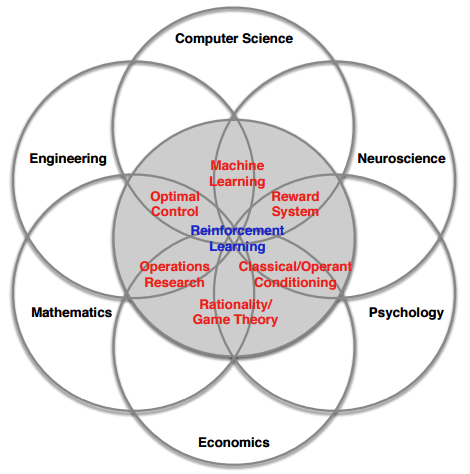
\includegraphics[width=8cm]{./pic/introduction/diagram.png}
\centering
\caption{Many faces of reinforcement learning}
\end{figure}

RL is a framework for general learning and is said to be the general artificial intelligent. The main components of reinforcement learning consist of agent, environment and reward. An agent is an actor who acts inside a given environment with the main purpose to maximize the reward that is given by the environment. For example, a dog (agent) obeys its owner (environment) command in order to have some food (reward) or a robot (agent) trying to solve the maze (environment) so that it can exit the maze as soon as possible (reward).

\begin{figure}[h]
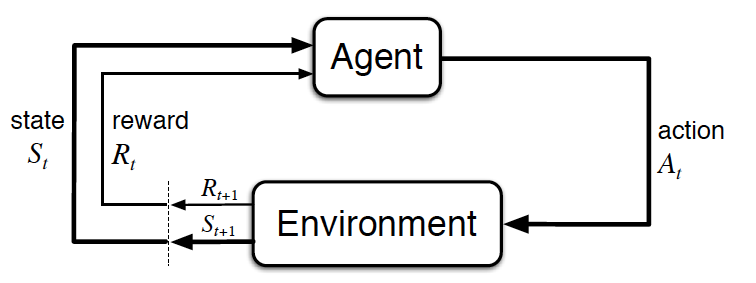
\includegraphics[width=8cm]{./pic/introduction/Sutton}
\centering
\caption{Reinforcement learning}
\end{figure}

The agent observes the consequence of its action from the environment. These observation can be considered as a state of an agent. The agent observes its state, which can be partially observable or need to be estimated from any information that it can acquire, then choose the optimal action that can lead them to maximize its reward. Terminal state can be defined as the last state that the agent is in before exiting the environment.    

We can model RL as Markov Decision Process (MDP) where each state could be transited to other states with according to action taken by the agent. This state transition at time $t+1$ can be written as $p(s_{t+1}|{a_t},{s_t})$ and the agent will receive a reward of $r_t$ which can be positive or negative. At terminal state, the transition probability for all possible actions are 1 i.e. $p(s_{Terminal}|{a_t},s_{Terminal}) = 1$ and the reward at this state will always be $0$.

\begin{figure}[h]
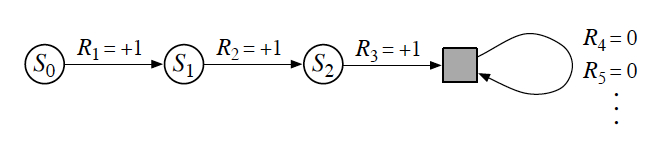
\includegraphics[width=8cm]{./pic/introduction/MDP}
\centering
\caption{MDP}
\end{figure}

There are two kind of reward in RL community. The first one is, immediate reward, the reward that the agent will immediately receive after each action. The second reward is a reward that the agent does not receive right after the action but the action that the agent took, leads an agent to a good state for a higher reward. Take study as an example, you have a lower happiness level if you study during weekend on that week but you will have a higher happiness level later in your life because studying can lead you to a better career and higher fortune. 


The latter reward can be written as a sum of expected reward that the agent will receive for being at a particular state multiply by discount rate. This means the reward that the agent received when he took an action at time step $t$ is $r_t + E[\gamma*r_{t+1}+\gamma^2*r_{t+2}+ ...]$ which is $r_t + \gamma*E[r_{t+1}+\gamma*r_{t+2}+ ...]$ or $$r_t + \gamma*V(s_{t+1})$$ where $r_t$ is the immediate reward at time step $t$ and $V(s_{t+1})$ is a Value function. The Value function is defined as an expected reward for being in state $s$ until the terminal state which can be further express as $$ V(s_{i+1}) = \Sigma_{i=t} \gamma^{i-t} \Sigma_{s'} \Sigma_a p(s_{i+1}'|a_{i},s_i)r_{i}  $$
One could write the value function as below to gain more intuitive. $$  V(s_t) = E_{a,s}[r_t] + \gamma V(s'_{t+1})  = E_{a,s}[r_t] + \gamma E_{a,s}[r_{t+1}] +\gamma^2 V(s'_{t+2})$$

Another important vocabulary in reinforcement learning is policy. Policy is defined as how agent chooses to act in a certain state, usually written as $\pi (a|s)$. A policy can be deterministic where $ a = \pi (a|s) = \pi(s)$ is a conditional statement or can be stochastic where $\pi (a|s) = P[a_t|s_t]$.

Lastly, the word model in RL refers to the model of predicting what the environment will do next. This means the transition probability $p(s_{i+1}'|a_{i},s_i)$ is fully known or can be infer. Also the expected reward of each step $E[r_{t+1}|s_t, a_t]$ is known.

Before we drive into the algorithm using to solve RL problem, the definition of action-value function should be derived. Action-value function , sometime known as Q-value, denoted as $Q(s,a)$ is an expected accumulated reward of agent being at state $s$ and taking action $a$. Thus the action-value function can be derived as $$ Q_{\pi}(s,a) = E[\Sigma_{t=0} \gamma^t r_{t+1}| s_t, a_t ]$$  where $\pi$ is a policy of the agent.


\section{Solving reinforcement learning problem}
 
In this section, we describe approaches for solving reinforcement learning problem. The goal of reinforcement problem is to discover an optimal policy $\pi^*(a|s)$ that maps states to action so as to maximize the expected cumulative reward, $E[\Sigma^\infty_{t=0} \gamma^t r_t]$. In some setting, the episode may end after time step $T$ and the environment is reset so do the agent. This kind of task is called an episodic task.

In contrast of supervised learning where labeled training data is already given to train the model, reinforcement learning algorithm learn to maximize the reward by collecting the data in order to feed into the learning algorithm. The agent collects that data by exploring the environment to receive data for learning the correlation between action and reward. This trade-off between exploring and exploiting is known as explore and exploit dilemma. The agent must choose between exploiting the environment by greedily choose the action that leads to maximize the reward or exploring the environment to gain more information about it. 

Two types of policy are Off-policy method and On-policy method. Off-policy method learns independent of the employed policy i.e. an explorative strategy that is different from the desired final policy can be employed during the learning process. On-policy method collects sample information about the environment using the current policy.
  
\subsection{Temporal Difference learning}

Temporal difference learning or TD learning is one of the update algorithm that use in learning in RL. Classically problem like reinforcement learning can be treat by using approach from dynamic programming (DP) or Monte Carlo (MC) method. TD learning can be thought as a method in between DP and MC.Like Monte Carlo methods, TD methods can learn directly from raw experience without a model of the environment's dynamics. Like DP, TD methods update estimates based in part on other learned estimates, without waiting for a final outcome (bootstrap).

TD prediction updates the value function of each state in order to estimate the true value function based on the receiving reward during the episode according to the policy that the agent obey. The simplest TD method makes the update immediately on transition to $S_{t+1}$ and receiving $R_{t+1}$ as
$$ V(S_t) \leftarrow V(S_t) + \alpha[(r_{t+1} + \gamma V(S_{t+1}) - V(S_t))].$$ where $\alpha$ is the learning rate. 

\begin{algorithm}
\caption{TD learning}\label{TD learning}
\begin{algorithmic}[1]
\State Input: Policy that we choose to evaluate $\pi$
\State Initialize $V(s)$ arbitrarily 
\State \emph{Repeat (for each episode)}:
\State \indent Initialize S
\State \indent Repeat (for each step in episode):
\State \indent \indent A $\leftarrow$ action given by $\pi$ for $S$
\State \indent \indent Take action A, observe R, S'   
\State \indent \indent V(s) $\leftarrow$ V(s) + $\alpha$[r + $\gamma V(s') - V(s)$ ]
\State \indent \indent S $\leftarrow$ S'
\State \indent Until S is terminal
\end{algorithmic}
\end{algorithm}

The optimal policy is the policy that has a higher value function for every state or $\pi^*$ is optimal policy if and only if $V_{\pi^*}(s) \geq V_{\pi}(s)$ for all $s \in S$ and $\pi$ in all possible policy.

TD learning can also be applied to state-action value function. The state-action value function is updated as $$ Q(S_t, a_t) \leftarrow Q(S_t, a_t) + \alpha[(r_{t} + \gamma Q(S_{t+1},a_{t+1}) - Q(S_t,a_t))].$$

\subsection{Discrete state space discrete action space problem}





\end{document}